\documentclass[11pt]{article} %[12pt]

\usepackage[utf8]{inputenc}
\usepackage[T1]{fontenc}
\usepackage{lmodern}
\usepackage[english]{babel}
\usepackage{amsmath}
\usepackage{listings}
\usepackage{graphicx}
\usepackage{enumitem}
\usepackage{amssymb}
\usepackage{verbatim}
\usepackage{pdfpages}
\usepackage{algpseudocode}
\usepackage{breqn}
\usepackage[linesnumbered,ruled,vlined]{algorithm2e}
\usepackage{tikz}
\usetikzlibrary{positioning,shapes.multipart}
\usepackage{textcomp}
\SetArgSty{textup}
\usepackage{fancyhdr}

\topmargin -2cm 
\textheight 24cm
\textwidth 16.0 cm 
\oddsidemargin -0.1cm

 
 \pagestyle{fancy}
 \fancyhf{}
 \fancyhead[LE,RO]{Exercise 2}
 \fancyhead[RE,LO]{Deep Learning for Computer Vision}
 \fancyfoot[CE,CO]{\leftmark}
 \fancyfoot[LE,RO]{\thepage}

\newcommand{\R}{\mathbb{R}}
\newcommand{\E}{\mathbb{E}}
\newcommand{\Var}{\mathrm{Var}}
\newcommand{\N}{\mathbb{N}}
\newcommand{\Q}{\mathbb{Q}}
\newcommand{\C}{\mathbb{C}}
\newcommand{\Z}{\mathbb{Z}}
\newcommand{\ggT}{\text{ggT}}
\newcommand{\kgV}{\text{kgV}}
\newcommand{\spa}[1]{\; #1 \;}
\newcommand{\bewbeh}[2]{\begin{enumerate} \item[\textbf{Beh.}]#1 \item[\textbf{Bew.}]#2
	\end{enumerate}}
\newcommand{\induct}[2]{\begin{enumerate} \item[\textit{IA}]#1 \item[\textit{IS}]#2
	\end{enumerate}}
\newcommand{\qed}{\hfill\ensuremath{\square}}
\newcommand{\gdw}[2]{\begin{enumerate} \item[$\Rightarrow$]#1 \item[$\Leftarrow$]#2
	\end{enumerate}}
\newcommand{\intsto}[1]{\{1, \dots, #1\}}
\newcommand\Item[1][]{%
	\ifx\relax#1\relax  \item \else \item[#1] \fi
	\abovedisplayskip=0pt\abovedisplayshortskip=0pt~\vspace*{-\baselineskip}}



\begin{document}
\section*{Exercise 2.1 c}
\begin{figure}[htb]
  \centering
  \centerline{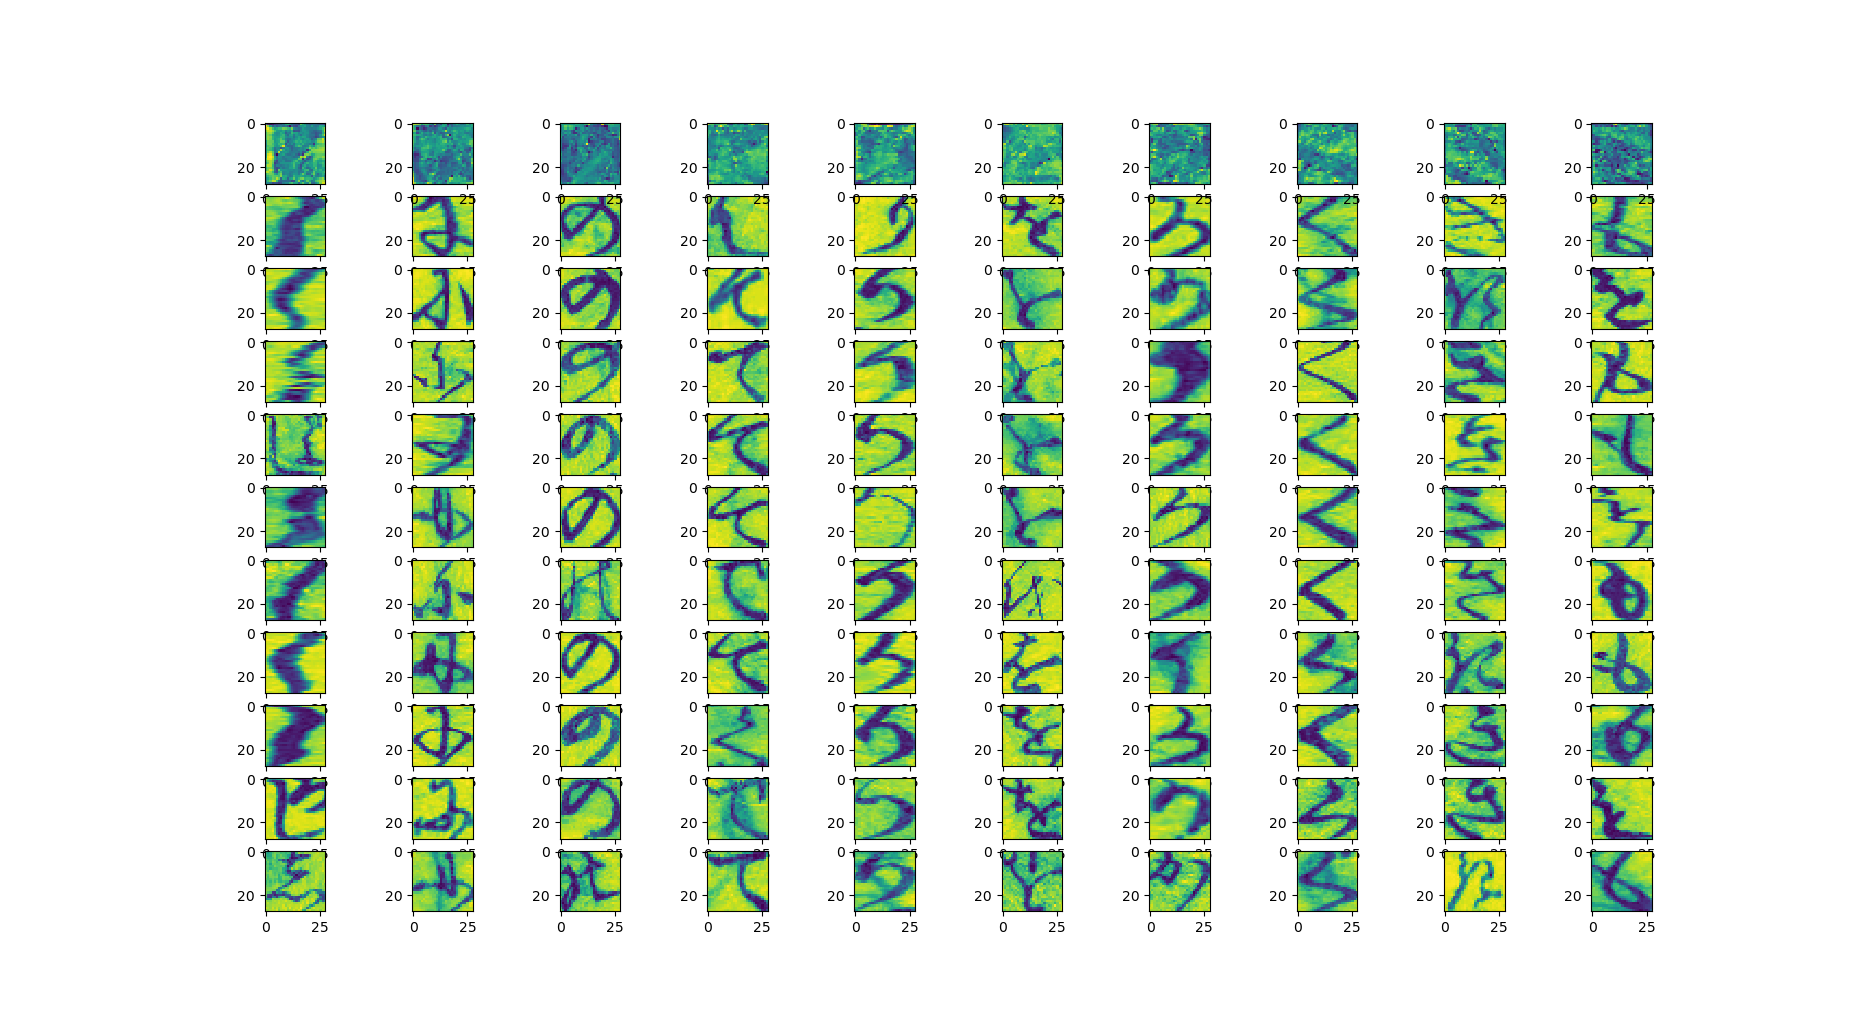
\includegraphics[width=1.35\textwidth ]{Figure_1_1.png}}
  \vspace{-5pt}
    \centering
\caption{Visualization of the weights vectors and example data images. The darker parts in the visualization of the weights vectors look similar to the real example images.}
\vspace{-1pt}
\end{figure}
\clearpage

\section*{Exercise 2.2}
\begin{figure}[htb]
  \centering
  \centerline{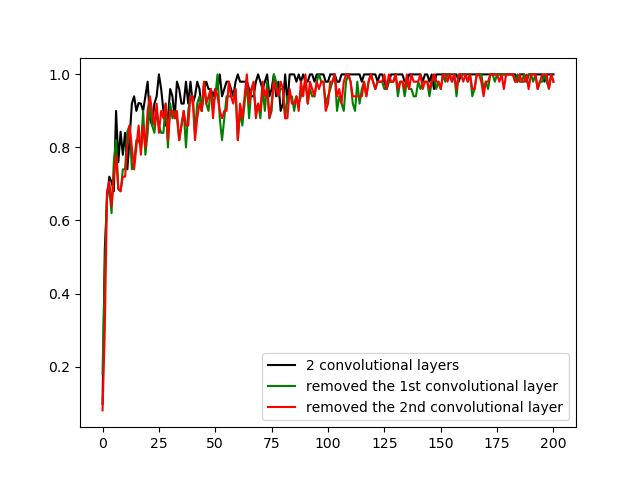
\includegraphics[width=1\textwidth ]{Figure_2_4.png}}
  \vspace{-5pt}
    \centering
\caption{(d). Visualization of training accuracies while removing convolutional layers. Removing each convolutional layers increases the number of parameters. If we remove the first layer, the convolutional layer will have 64 feature maps; if we remove the second layer, it still have 64 feature maps. But no matter which layer is removed, since a max-pooling operation is also missing, the feature maps' size become twice of that with two layers and two max-pooling operations. From the figure we can see that the training accuracies with only one convolutional layer are lower than that with both layers. The test accuracy with both convolutional layer is around 97\%, only with the 1st layer is around 95.1\% and only with the 2nd layer is around 95.2\%. Additionally, the training time only with the 2nd convolutional layer is apparently longer than only with the 1st convolutional layer.}
\vspace{-1pt}
\end{figure}

\begin{figure}[htb]
  \centering
  \centerline{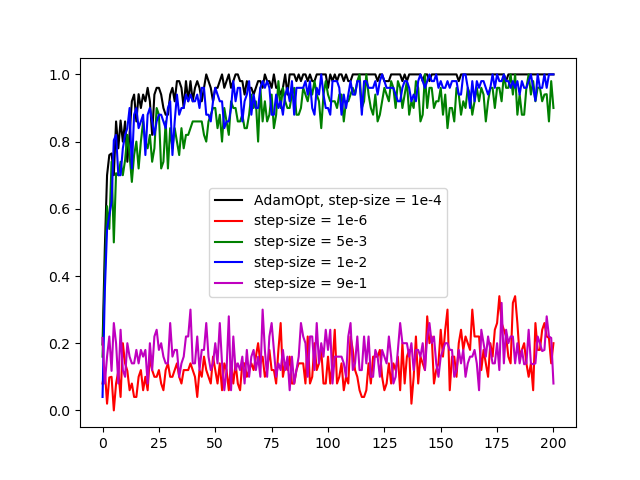
\includegraphics[width=1\textwidth ]{Figure_2_5.png}}
  \vspace{-5pt}
    \centering
\caption{(e). Visualization of training accuracies with changing the step size. Too small step size will make the gradient descent progress so slowly that within the iterations it cannot reach or come out of a local minimum; Too large step size will make the gradient descent travel between two sides of a (local) minimum and never reach it.}
\vspace{-1pt}
\end{figure}
\clearpage

\begin{figure}[htb]
  \centering
  \centerline{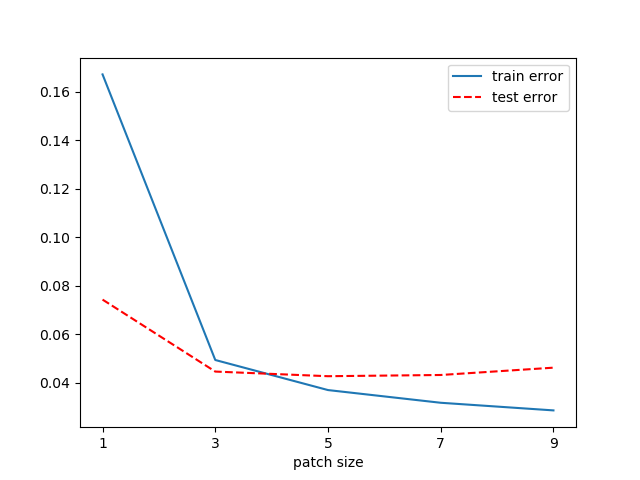
\includegraphics[width=1\textwidth ]{hyper_patch_size.png}}
  \vspace{-5pt}
    \centering
\caption{(f). Visualization of 5-folds cross validation training and test accuracies with changing the patch size. The patch size candidates are 1, 3, 5, 7 and 9. From the figure we could say that the patch size = 3 might be a better choice.}
\vspace{-1pt}
\end{figure}

\begin{figure}[htb]
  \centering
  \centerline{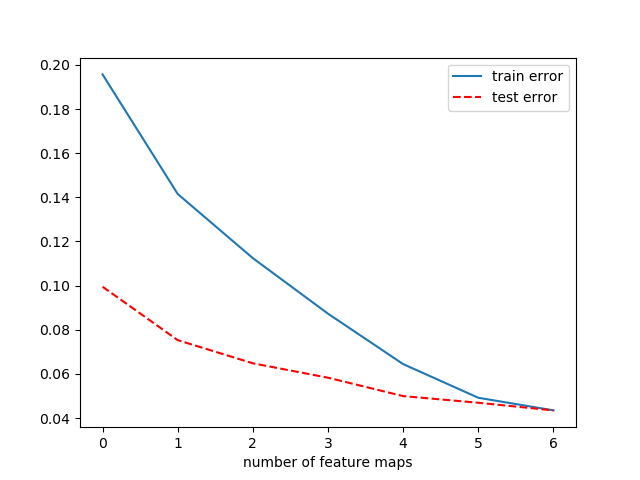
\includegraphics[width=1\textwidth ]{feature_map.png}}
  \vspace{-5pt}
    \centering
\caption{(f). Visualization of 5-folds cross validation training and test accuracies with changing the number of feature maps. The number of feature maps goes from $2^{0}$ to $2^{6}$. Assume that the 2nd layer has twice the feature maps as the 1st layer. From the figure we could see that $2^{6}$ is exactly the turning point to over-fitting. So the kernel size of the convolutionnal layers is $3 \times 3$ and the 1st layer has $2^{6}$ feature maps and the 2nd has $2^{7}$.}
\vspace{-1pt}
\end{figure}
\clearpage

\section*{Exercise 2.3}

\begin{figure}[htb]
  \centering
  \centerline{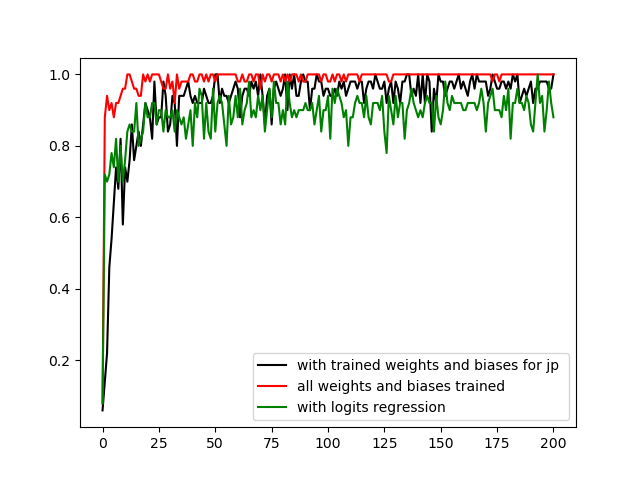
\includegraphics[width=1\textwidth ]{Figure_3.png}}
  \vspace{-5pt}
    \centering
\caption{Visualization of training MNIST with different strategies.}
\vspace{-1pt}
\end{figure}
\clearpage

\section*{Exercise 2.5}
\begin{enumerate}[label= (\alph*) \;]
  \item $ \displaystyle
    \E(\bar x) = \E\Big( \frac 1 L \sum_{l=1}^L x_l \Big)
    = \frac 1 L \sum_{l=1}^L \E(x_l)
    = \frac 1 L \sum_{l=1}^L \frac \theta 2
    = \frac \theta 2$

  \item With $\hat x := 2 \bar x$ it is
    $\E(\hat x) = \E(2 \bar x) = 2 \E(\bar x) = \theta$.

  \item The standard error
    \[ \displaystyle
      \E((\hat x - \theta)^2)
      = \E((\hat x - \E(\hat x))^2)
      = \Var(\hat x)
      = \Var\Big( \frac 2 n \sum_{l=1}^L x_l \Big)
      = \frac{4}{L^2} \sum_{l=1}^L \Var(x_l)
      = \frac 4 L \Var(x_1)
    \]
    clearly goes to zero for $L \to \infty$.

  \item Let $\tilde x := \hat x + \frac 1 L$. It is
    \[
      \E(\tilde x)
      = \E(\hat x + \frac 1 L)
      = \theta + \frac 1 L
    \]
    and
    \[
      \E((\tilde x - \theta)^2)
      = \E((\hat x + \frac 1 L - \theta)^2)
      = \E((\hat x - \theta)^2 + \frac{1}{L^2} + \frac 2 L (\hat x - \theta))
      = \frac 4 L \Var(x_1) + \frac{1}{L^2}
    \]
    which goes to zero for $L \to \infty$.
\end{enumerate}

\end{document}
